\chapter{通过真核生物 RNA-Seq 数据估计基因的转录组问题为 NP 难}
\label{chap-rna-seq-nphard}

\section{问题描述}
在真核生物 RNA-Seq 数据处理过程当中, 重要的一步是通过 RNA-Seq 数据估计出基因的转录组. 
由于在真核生物的转录过程当中会有选择性剪切的现象发生, 一个基因可能转录出多个剪切异构体. 
在这种情况下, 我们需要通过 RNA-Seq 数据估计出转录本的组成. 
在这里我们首先对通过真核生物 RNA-Seq 数据估计基因的转录组的问题, 
亦即对基因的剪切异构体的辨识, 进行描述. 

在 RNA-Seq 实验中得到的读段数据在比对到参考基因组序列上如图 \ref{nphard.ex1.aligned.data} 所示. 
对于 RNA-Seq 数据, 
我们可以通过序列拼装工具 (例如 Trinity \cite{grabherr2011full} 等) 进行拼装. 
得到每一个基因的外显子的序列以及这些外显子之间是如何连接在一起的关系, 
从而得到每一个基因的剪切图 \cite{Heber01072002}. 
在有基因的参考序列以及基因注释的情况下, 也可以直接通过基因注释获得每一个基因的剪切图. 
对于图 \ref{nphard.ex1.aligned.data} 中所示的基因和 RNA-Seq 数据, 
通过 Trinity 拼装获得的剪切图如图 \ref{nphard.ex1.splicing.graph} 所示. 

\begin{figure}[!t]
\centering
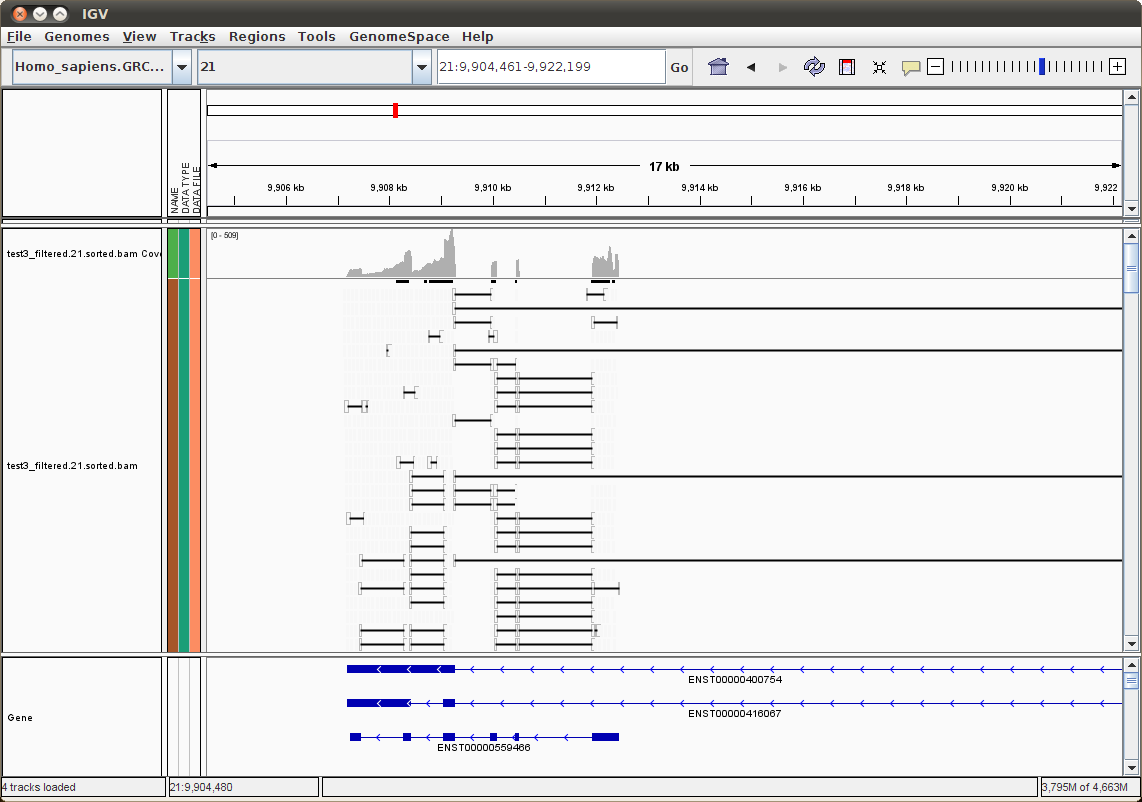
\includegraphics[width=\textwidth]{figures/nphard/comp1.png}
\caption{一个基因的比对到基因组参考序列上的 RNA-Seq 数据}
\label{nphard.ex1.aligned.data}
\end{figure}

\begin{figure}[!t]
\centering
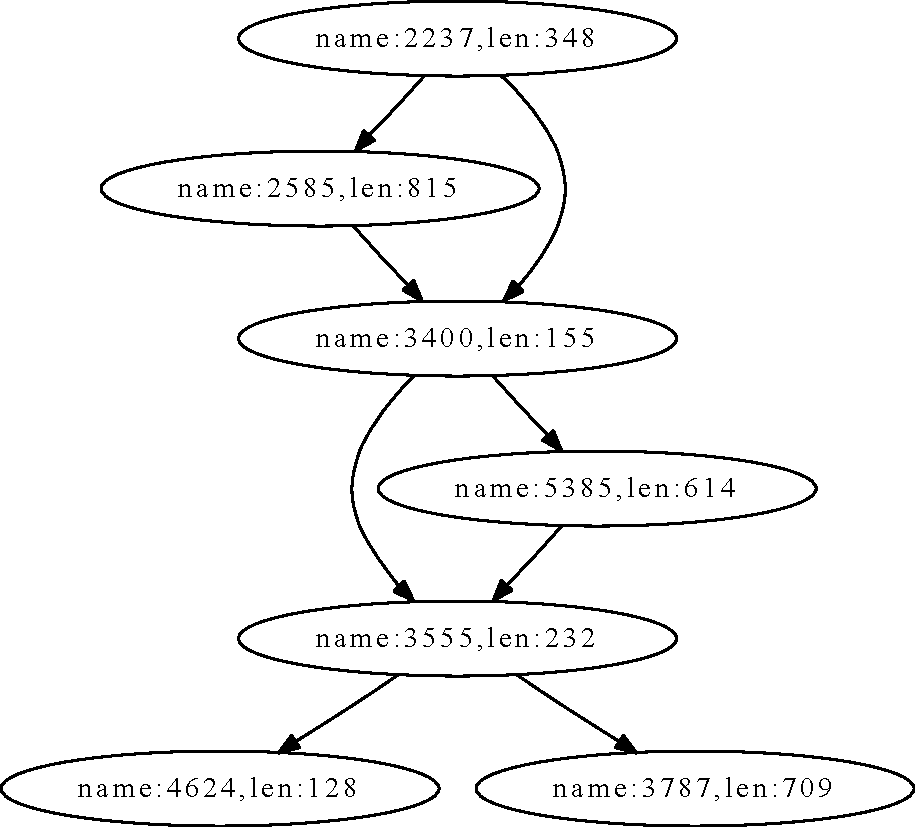
\includegraphics[width=\textwidth]{figures/nphard/comp1.pdf}
\caption{图 \ref{nphard.ex1.aligned.data} 中所示的基因和 
RNA-Seq 数据通过 Trinity \cite{grabherr2011full} 拼装得到的剪切图}
\label{nphard.ex1.splicing.graph}
\end{figure}

\subsection{模型}

为了能够通过 RNA-Seq 数据估计出转录组中转录本的组成, 辨识每个基因的剪切异构体, 
我们在这里介绍一个 Poisson 模型用来描述 RNA-Seq 数据 \cite{Jiang15042009}. 
该模型与 \ref{rna-seq-general-model} 中所介绍的多项式模型在数学上是等价的 
\cite{2011arXiv1104.3889P}. 
在这里采用 RNA-Seq 数据的 Poisson 模型是为了简化问题的描述. 

另外, 为了叙述的方便, 我们在这里纸考虑辨识一个基因的剪切异构体. 

对于真核生物中的一个基因, 根据剪切图的定义, 
我们将其表示为一个有向无环图 $G=(V,E)$, 其中 $G$ 中的一个节点代表一个外显子, 
节点 $v_i$ 到 $v_j$ 有一条边当且仅当在这个基因当中有一个剪切异构体同时包含 
$v_i$ 和 $v_j$ 所代表的外显子, 
同时在这个剪切异构体中 $v_i$ 和 $v_j$ 所代表的外显子是相邻的, 
并且 $v_i$ 代表的外显子在 $v_j$ 代表的外显子的 5' 上端. 

该基因的一个剪切异构体是图 $G$ 中的一个路径 $v_1 \to v_2 \to \ldots \to v_k$, 
其中 $v_i$, $i=1,2,\ldots,k$ 是构成该剪切异构体的外显子. 
我们用 $I$ 表示这个基因的剪切异构体构成的集合, $\lambda_i \geq 0$, 
$i \in I$ 是剪切异构体 $i$ 的表达量. 

在这里, 我们假设所有的 RNA-Seq 数据均是单端读段, 且长度均为 $k$. 
(对于长度不均的读段或者双端测序的读段我们可以采用与这里类似的方法进行处理, 
此处不再赘述, 感兴趣的读者可以参看 \onlinecite{cufflinks.2010}) 
一个读段对应到剪切图中时, 该读段对应到原转录本上的每一个外显子在剪切图中所对应的节点, 
同时在读段经过多个外显子时该读段也会经过剪切图中所对应的边. 
为了描述的方便, 我们把每一个读段对应在原转录本上的 5' 端的位置称之为该读段的起始位置, 
对应在原转录本上的 3' 端的位置称之为该读段的终止位置. 

我们假设每一个读段可以在该基因中的位置是已知的并且是唯一的 
(对于基因序列的分析表明这样一个假设是合理的 \cite{peng2011t}). 

同时, 我们把该基因在 RNA-Seq 实验中所有对应的读段构成的集合记为 $R$. 

在用来描述 RNA-Seq 数据的 Poisson 模型中, 
我们假设对于基因中的每一个位置 $p$, 
在这个位置起始的读段的个数满足参数为 
\[
\sum_{\text{剪切异构体 $i \in I$ 经过该位置}} a_{pi} \lambda_i
\]
的 Poisson 分布. (此处可以参考图 \ref{nphard.ex1.aligned.data} 进行理解.)
这里 $a_{pi} \geq 0$ 是与目前该位置 $p$ 有关的一个采样率 \cite{2011arXiv1106.3211S}. 
我们假设在给定基因中的一个位置 $p$ 之后, 以及一个剪切异构体 $i \in I$, 
$a_{pi}$ 是已知的. 
对于理想的情况我们认为对于所有的基因中的位置 $p$ 和剪切异构体 $i\in I$, 
我们均有 $a_{pi}=1$. 
通过不同的位置和不同的剪切异构体 $i\in I$ 的 $a_{pi}$, 
我们可以对 RNA-Seq 实验中存在的不均匀性进行建模. 
为了方便下面的陈述, 我们记基因中所有可以有读段起始的位置的集合记作 $P$. 
(例如, 对于一个只有一个外显子的基因, 其长度为 $L$, 
$P$ 由该基因上的前 $L-k+1$ 个位置组成.)

同时, 我们假设对于该基因中不同的位置, 
在这些位置起始的读段的个数的分布式独立的. 

\subsection{M-ISOFORM 判定问题}

\section{证明}

